% -*- TeX-engine: xetex; eval: (auto-fill-mode 0); eval: (visual-line-mode 1); -*-
% Compile with XeLaTeX

%%%%%%%%%%%%%%%%%%%%%%%
% To do before class
%%%%%%%%%%%%%%%%%%%%%%%

% Send the Logistics/Week0Annoucnement (the night before).
% Send an email reminding students to bring a charged computer (the night before).

%%%%%%%%%%%%%%%%%%%%%%%
% Option 1: Slides: (comment for handouts)   %
%%%%%%%%%%%%%%%%%%%%%%%

\documentclass[slidestop,compress,mathserif,12pt,t,professionalfonts,xcolor=table]{beamer}

% solution stuff
\newcommand{\solnMult}[1]{
\only<1>{#1}
\only<2->{\red{\textbf{#1}}}
}
\newcommand{\soln}[1]{\textit{#1}}

\newcommand{\solnMultOn}[3]{
\only<#1>{#3}
\only<{#2}->{\red{\textbf{#3}}}
}

%%%%%%%%%%%%%%%%%%%%%%%%%%%%%%%
% Option 2: Handouts, without solutions (post before class)    %
%%%%%%%%%%%%%%%%%%%%%%%%%%%%%%%

% \documentclass[11pt,containsverbatim,handout,xcolor=xelatex,dvipsnames,table]{beamer}

% % handout layout
% \usepackage{pgfpages}
% \pgfpagesuselayout{4 on 1}[letterpaper,landscape,border shrink=5mm]

% % solution stuff
% \newcommand{\solnMult}[1]{#1}
% \newcommand{\soln}[1]{}
% \newcommand{\solnMultOn}[3]{#3}

% % % This breaks things for me for some reason.
% % tell pgfpages how to set page sizes in XeLaTeX
% %\renewcommand\pgfsetupphysicalpagesizes{%
% %   \pdfpagewidth\pgfphysicalwidth\pdfpageheight\pgfphysicalheight%
% %}

%%%%%%%%%%%%%%%%%%%%%%%%%%%%%%%%%%%%
% Option 3: Handouts, with solutions (may post after class if need be)    %
%%%%%%%%%%%%%%%%%%%%%%%%%%%%%%%%%%%%

% \documentclass[11pt,containsverbatim,handout,xcolor=xelatex,dvipsnames,table]{beamer}

% % handout layout
% \usepackage{pgfpages}
% \pgfpagesuselayout{4 on 1}[letterpaper,landscape,border shrink=5mm]

% % solution stuff
% \newcommand{\solnMult}[1]{\red{\textbf{#1}}}
% \newcommand{\soln}[1]{\textit{#1}}

% % % This breaks things for me for some reason.
% % % tell pgfpages how to set page sizes in XeLaTeX
% % \renewcommand\pgfsetupphysicalpagesizes{%
% %    \pdfpagewidth\pgfphysicalwidth\pdfpageheight\pgfphysicalheight%
% % }

%%%%%%%%%%%%%%%%%%%%%%%%%%%%%%%
% Option 4: Notes Only
%%%%%%%%%%%%%%%%%%%%%%%%%%%%%%%

% % See http://tex.stackexchange.com/questions/11421/add-notes-to-latex-beamer
% \documentclass[10pt,containsverbatim,xcolor=xelatex,dvipsnames,table,notes=only]{beamer}

% % handout layout
% % \usepackage{pgfpages}
% % \pgfpagesuselayout{1 on 1}[letterpaper, landscape, border shrink=5mm]

% % solution stuff
% \newcommand{\solnMult}[1]{#1}
% \newcommand{\soln}[1]{}

% % % Having a problem with this.
% % tell pgfpages how to set page sizes in XeLaTeX
% % \renewcommand\pgfsetupphysicalpagesizes{%
% %   \pdfpagewidth\pgfphysicalwidth\pdfpageheight\pgfphysicalheight%
% %}

%%%%%%%%%%
% Load style file, defaults  %
%%%%%%%%%%

%%%%%%%%%%%%%%%%
% Themes
%%%%%%%%%%%%%%%%

% See http://deic.uab.es/~iblanes/beamer_gallery/ for mor options

% Style theme
\usetheme{Pittsburgh}

% Color theme
\usecolortheme{seahorse}

% Helvetica Neue Light for most text
\usepackage{fontspec}
\setsansfont{Helvetica Neue Light}

%%%%%%%%%%%%%%%%
% Packages
%%%%%%%%%%%%%%%%

\usepackage{geometry}
\usepackage{graphicx}
\usepackage{amssymb}
\usepackage{epstopdf}
\usepackage{amsmath}  	% this permits text in eqnarray among other benefits
\usepackage{url}		% produces hyperlinks
\usepackage[english]{babel}
\usepackage{colortbl}	% allows for color usage in tables
\usepackage{multirow}	% allows for rows that span multiple rows in tables
\usepackage{color}		% this package has a variety of color options
\usepackage{pgf}
\usepackage{calc}
\usepackage{ulem}
\usepackage{multicol}
\usepackage{textcomp}
\usepackage{listings}
\usepackage{changepage}
\usepackage{tikz}
\usetikzlibrary{trees}		% for probability trees
\usepackage{fancyvrb}	% for colored code chunks
\usepackage{nameref}

%%%%%%%%%%%%%%%%
% Remove navigation symbols
%%%%%%%%%%%%%%%%

\beamertemplatenavigationsymbolsempty
\hypersetup{pdfpagemode=UseNone} % don't show bookmarks on initial view

%%%%%%%%%%%%%%%%
% User defined colors
%%%%%%%%%%%%%%%%

% Pantone 2015 Spring colors
% http://iwork3.us/2014/09/16/pantone-2015-spring-fashion-report/
% update each semester or year

\xdefinecolor{custom_blue}{rgb}{0, 0.70, 0.79} % scuba blue
\xdefinecolor{custom_darkBlue}{rgb}{0.11, 0.31, 0.54} % classic blue
\xdefinecolor{custom_orange}{rgb}{0.97, 0.57, 0.34} % tangerine
\xdefinecolor{custom_green}{rgb}{0.49, 0.81, 0.71} % lucite green
\xdefinecolor{custom_red}{rgb}{0.58, 0.32, 0.32} % marsala

\xdefinecolor{custom_lightGray}{rgb}{0.78, 0.80, 0.80} % glacier gray
\xdefinecolor{custom_darkGray}{rgb}{0.54, 0.52, 0.53} % titanium

%%%%%%%%%%%%%%%%
% Template colors
%%%%%%%%%%%%%%%%

\setbeamercolor*{palette primary}{fg=white,bg= custom_blue}
\setbeamercolor*{palette secondary}{fg=black,bg= custom_blue!80!black}
\setbeamercolor*{palette tertiary}{fg=white,bg= custom_blue!80!black!80}
\setbeamercolor*{palette quaternary}{fg=white,bg= custom_blue}

\setbeamercolor{structure}{fg= custom_blue}
\setbeamercolor{frametitle}{bg= custom_blue!90}
\setbeamertemplate{blocks}[shadow=false]
\setbeamersize{text margin left=2em,text margin right=2em}

%%%%%%%%%%%%%%%%
% Styling fonts, bullets, etc.
%%%%%%%%%%%%%%%%

% title slide
\setbeamerfont{title}{size=\large,series=\bfseries}
\setbeamerfont{subtitle}{size=\large,series=\mdseries}
%\setbeamerfont{institute}{size=\large,series=\mdseries}

% color of alerted text
\setbeamercolor{alerted text}{fg=custom_orange}

% styling of itemize bullets
\setbeamercolor{item}{fg=custom_blue}
\setbeamertemplate{itemize item}{{{\small$\blacktriangleright$}}}
\setbeamercolor{subitem}{fg=custom_blue}
\setbeamertemplate{itemize subitem}{{\textendash}}
\setbeamerfont{itemize/enumerate subbody}{size=\footnotesize}
\setbeamerfont{itemize/enumerate subitem}{size=\footnotesize}

% styling of enumerate bullets
\setbeamertemplate{enumerate item}{\insertenumlabel.}
\setbeamerfont{enumerate item}{family={\fontspec{Helvetica Neue}}}
\setbeamerfont{enumerate subitem}{family={\fontspec{Helvetica Neue}}}
\setbeamerfont{enumerate subsubitem}{family={\fontspec{Helvetica Neue}}}

% make frame titles small to make room in the slide
\setbeamerfont{frametitle}{size=\small} 

% set Helvetica Neue font for frame and section titles
\setbeamerfont{frametitle}{family={\fontspec{Helvetica Neue}}}
\setbeamerfont{sectiontitle}{family={\fontspec{Helvetica Neue}}}
\setbeamerfont{section in toc}{family={\fontspec{Helvetica Neue}}}
\setbeamerfont{subsection in toc}{family={\fontspec{Helvetica Neue}}, size=\small}
\setbeamerfont{footline}{family={\fontspec{Helvetica Neue}}}
\setbeamerfont{subsection in toc}{family={\fontspec{Helvetica Neue}}}
\setbeamerfont{block title}{family={\fontspec{Helvetica Neue}}}

%%%%%%%%%%%%%%%%
% New fonts accessed by fontspec package
%%%%%%%%%%%%%%%%

% Monaco font for code
\newfontfamily{\monaco}{Monaco}

%%%%%%%%%%%%%%%%
% Color text commands
%%%%%%%%%%%%%%%%

%orange
\newcommand{\orange}[1]{\textit{\textcolor{custom_orange}{#1}}}

% green
\newcommand{\green}[1]{\textit{\textcolor{custom_green}{#1}}}

% red
\newcommand{\red}[1]{\textit{\textcolor{custom_red}{#1}}}

% dark gray
\newcommand{\darkgray}[1]{\textit{\textcolor{custom_darkGray}{#1}}}

% light gray
\newcommand{\lightgray}[1]{\textit{\textcolor{custom_lightGray}{#1}}}

% pink
\newcommand{\pink}[1]{\textit{\textcolor{pink}{#1}}}


%%%%%%%%%%%%%%%%
% Custom commands
%%%%%%%%%%%%%%%%

% empty box for probability tree frame
\newcommand{\emptybox}[2]{
	\fbox{ \begin{minipage}{#1} \hfill\vspace{#2} \end{minipage} }
}

% cancel
\newcommand{\cancel}[1]{%
    \tikz[baseline=(tocancel.base)]{
        \node[inner sep=0pt,outer sep=0pt] (tocancel) {#1};
        \draw[red, line width=0.5mm] (tocancel.south west) -- (tocancel.north east);
    }%
}

% degree
\newcommand{\degree}{\ensuremath{^\circ}}

% cite
\newcommand{\ct}[1]{
\vfill
{\tiny #1}}

% Note
\newcommand{\Note}[1]{
\rule{2.5cm}{0.25pt} \\ \textit{\footnotesize{\textcolor{custom_red}{Note:} \textcolor{custom_darkGray}{#1}}}}

% Remember
\newcommand{\Remember}[1]{\textit{\scriptsize{\textcolor{custom_red}{Remember:} #1}}}

% links: webURL, webLink
\newcommand{\webURL}[1]{\urlstyle{same}{\textit{\textcolor{custom_blue}{\url{#1}}}}}
\newcommand{\webLink}[2]{\href{#1}{\textcolor{custom_blue}{{#2}}}}

% mail
\newcommand{\mail}[1]{\href{mailto:#1}{\textit{\textcolor{custom_blue}{#1}}}}

% highlighting: hl, hlGr, mathhl
\newcommand{\hl}[1]{\textit{\textcolor{custom_blue}{#1}}}
\newcommand{\hlGr}[1]{\textit{\textcolor{custom_green}{#1}}}
\newcommand{\mathhl}[1]{\textcolor{custom_blue}{\ensuremath{#1}}}

% example
\newcommand{\ex}[1]{\textcolor{blue}{{{\small (#1)}}}}

% two col: two columns
\newenvironment{twocol}[4]{
\begin{columns}[c]
\column{#1\textwidth}
#3
\column{#2\textwidth}
#4
\end{columns}
}

% slot (for probability calculations)
\newenvironment{slot}[2]{
\begin{array}{c} 
\underline{#1} \\ 
#2
\end{array}
}

% pr: left and right parentheses
\newcommand{\pr}[1]{
\left( #1 \right)
}

%%%%%%%%%%%%%%%%
% Custom blocks
%%%%%%%%%%%%%%%%

% activity: less commonly used
\newcommand{\activity}[2]{
\setbeamertemplate{itemize item}{{{\small\textcolor{custom_orange}{$\blacktriangleright$}}}}
\setbeamercolor{block title}{fg=white, bg=custom_orange}
\setbeamerfont{block title}{size=\small}
\setbeamercolor{block body}{fg=black, bg=custom_orange!20!white!80}
\setbeamerfont{block body}{size=\small}
\begin{block}{Activity: #1}
\setlength\abovedisplayskip{0pt}
#2
\end{block}
}

% app: application exercise
\newcommand{\app}[2]{
\setbeamercolor{block title}{fg=white,bg=custom_green}
\setbeamercolor{block body}{fg=black,bg=custom_green!20!white!80}
\begin{block}{{\small Application exercise: #1}}
#2
\end{block}
}

% disc: discussion question
\newcommand{\disc}[1]{
\vspace*{-2ex}
\setbeamercolor{block body}{bg=custom_blue!25!white!80, fg=custom_blue!55!black!95}
\begin{block}{\vspace*{-3ex}}
#1
\end{block}
\vspace*{-1ex}
}

% clicker: clicker question
\newcommand{\clicker}[1]{
\setbeamercolor{block title}{bg=custom_blue!80!white!50,fg=custom_blue!30!black!90}
\setbeamercolor{block body}{bg=custom_blue!20!white!80,fg=custom_blue!30!black!90}
\begin{block}{\vspace*{-0.2ex}{\footnotesize Clicker question}\vspace*{-0.2ex}}
#1
\end{block}
}

% formula
\newcommand{\formula}[2]{
\setbeamercolor{block title}{bg=custom_blue!40!white!60,fg=custom_blue!55!black!95}
\begin{block}{{\small#1}}
#2
\end{block}
}

% code
\newcommand{\Rcode}[1]{
{\monaco {\footnotesize \textcolor{custom_darkBlue}{#1}}}
}

% output
\newcommand{\Rout}[1]{
{\monaco {\footnotesize \textcolor{custom_darkGray}{#1}}}
}

%%%%%%%%%%%%%%%%
% Change margin
%%%%%%%%%%%%%%%%

\newenvironment{changemargin}[2]{%
\begin{list}{}{%
\setlength{\topsep}{0pt}%
\setlength{\leftmargin}{#1}%
\setlength{\rightmargin}{#2}%
\setlength{\listparindent}{\parindent}%
\setlength{\itemindent}{\parindent}%
\setlength{\parsep}{\parskip}%
}%
\item}{\end{list}}

%%%%%%%%%%%%%%%%
% Footnote
%%%%%%%%%%%%%%%%

\long\def\symbolfootnote[#1]#2{\begingroup%
\def\thefootnote{\fnsymbol{footnote}}\footnote[#1]{#2}\endgroup}

%%%%%%%%%%%%%%%%
% Graphics
%%%%%%%%%%%%%%%%

\DeclareGraphicsRule{.tif}{png}{.png}{`convert #1 `dirname #1`/`basename #1 .tif`.png}

%%%%%%%%%%%%%%%%
% Slide number
%%%%%%%%%%%%%%%%

\setbeamertemplate{footline}{%
    \raisebox{5pt}{\makebox[\paperwidth]{\hfill\makebox[20pt]{\color{gray}
          \scriptsize\insertframenumber}}}\hspace*{5pt}}

          
%%%%%%%%%%%%%%%%
% Remove page numbers
%%%%%%%%%%%%%%%%

\newcommand{\removepagenumbers}{% 
  \setbeamertemplate{footline}{}
}

%%%%%%%%%%%%%%%%
% TOC slides
%%%%%%%%%%%%%%%%

\setbeamertemplate{section in toc}{\inserttocsectionnumber.~\inserttocsection}
\setbeamertemplate{subsection in toc}{$\qquad$\inserttocsubsectionnumber.~\inserttocsubsection \\}

\AtBeginSection[] 
{ 
  \addtocounter{framenumber}{-1} 
  % 
  {\removepagenumbers 
  {\small
    \begin{frame}<beamer> 
    \frametitle{Outline} 
    \tableofcontents[currentsection] 
  \end{frame} 
  } 
  }
} 

\AtBeginSubsection[] 
{ 
  \addtocounter{framenumber}{-1} 
  % 
  {\removepagenumbers 
  {\small
    \begin{frame}<beamer> 
    \frametitle{Outline} 
    \tableofcontents[currentsection,currentsubsection] 
  \end{frame} 
  } 
  }
}
\input{../../definitions_default.tex}
% ALT ALT
%\input{../../definitions_custom.tex}

%%%%%%%%%%%
% Cover slide info    %
%%%%%%%%%%%

\title{Unit 5: Inference for categorical data}
\subtitle{2. Comparing two proportions}
\author{Sta 101 - Spring 2015}
\date{March 18, 2015}
\institute{Duke University, Department of Statistical Science}

%%%%%%%%%%%
% Begin document   %
%%%%%%%%%%%

\begin{document}

%%%%%%%%%%%%%%%%%%%%%%%%%%%%%%%%%%%%

% Title Page

\begin{frame}[plain]

\titlepage
\vfill
{\scriptsize \webLink{\PersonalSite}{Dr. \LastName{}} \hfill Slides posted at  \webLink{\CourseSite}{\CourseSite}}
\addtocounter{framenumber}{-1} 

\end{frame}

%%%%%%%%%%%%%%%%%%%%%%%%%%%%%%%%%%%%

\section{Housekeeping}

%%%%%%%%%%%%%%%%%%%%%%%%%%%%%%%%%%%%

\begin{frame}
\frametitle{Announcements}

\begin{itemize}

\item MT2 Review - Monday, March 23, 7-8pm

\item OH next week - Monday and Tuesday 3-5pm

\item MT review materials to be posted on Sakai over the weekend

\item RA5 opens on Sunday (but will also cover material from Monday's class so you might want to wait to take it) and will close at midnight on Monday

\item Mao's office hours moved to tomorrow 7-9pm, Tori is there tonight 7-9pm.

\end{itemize}

\end{frame}

%%%%%%%%%%%%%%%%%%%%%%%%%%%%%%%%%%%%

\section{Main ideas}

%%%%%%%%%%%%%%%%%%%%%%%%%%%%%%%%%%%%

\subsection{CLT also describes the distribution of $\hat{p}_1 - \hat{p}_2$}
\label{mi1}

%%%%%%%%%%%%%%%%%%%%%%%%%%%%%%%%%%%%

\begin{frame}
\frametitle{CLT also describes the distribution of $\hat{p}_1 - \hat{p}_2$}

\[ (\hat{p}_1 - \hat{p}_2) \sim N \pr{ mean = (p_1 - p_2), SE = \sqrt{ \frac{p_1(1-p_1)}{n_1} + \frac{p_2(1-p_2)}{n_2} } } \]

Conditions:
\begin{itemize}
\item Independence: Random sample/assignment + 10\% rule
\item Sample size / skew: At least 10 successes and failures
\end{itemize}

\end{frame}

%%%%%%%%%%%%%%%%%%%%%%%%%%%%%%%%%%%%

\subsection{For HT where $H_0: p_1 = p_2$, pool!}
\label{mi2}

%%%%%%%%%%%%%%%%%%%%%%%%%%%%%%%%%%%%

\begin{frame}
\frametitle{For HT where $H_0: p_1 = p_2$, pool!}

As with working with a single proportion,

\begin{itemize}

\item When doing a HT where $H_0: p_1 = p_2$ (almost always for HT), use expected counts / proportions for S-F condition and calculation of the standard error.

\item Otherwise use observed counts / proportions for S-F condition and calculation of the standard error.

\end{itemize}

\pause 

Expected proportion of success for both groups when $H_0: p_1 = p_2$ is defined as the \hl{pooled proportion}:
\[ \hat{p}_{pool} = \frac{total~successes}{total~sample~size} = \frac{suc_1 + suc_2}{n_1 + n_2} \]

\end{frame}

%%%%%%%%%%%%%%%%%%%%%%%%%%%%%%%%%%%%

\begin{frame}
\frametitle{}

\clicker{Suppose in group 1 30 out of 50 observations are successes, and in group 2 20 out of 60 observations are successes. What is the pooled proportion?}

\begin{enumerate}[(a)]
\item $\frac{30}{50}$
\item $\frac{20}{60}$
\item $\frac{30}{50} + \frac{20}{60}$
\item \solnMult{$\frac{30 + 20}{50 + 60}$}
\item $\frac{\frac{30}{50} + \frac{20}{60}}{2}$
\end{enumerate}

\end{frame}

%%%%%%%%%%%%%%%%%%%%%%%%%%%%%%%%%%%%

\subsection{When S-F fails, simulate!}
\label{mi3}

%%%%%%%%%%%%%%%%%%%%%%%%%%%%%%%%%%%%

\begin{frame}
\frametitle{When S-F fails, simulate!}

\begin{itemize}

\item If the S-F condition is met, can do theoretical inference: Z test, Z interval

\item If the S-F condition is not met, must use simulation based methods: randomization test, bootstrap interval

\end{itemize}

\end{frame}

%%%%%%%%%%%%%%%%%%%%%%%%%%%%%%%%%%%%

\section{Applications}

%%%%%%%%%%%%%%%%%%%%%%%%%%%%%%%%%%%%

\subsection{Two population proportions, small sample}

%%%%%%%%%%%%%%%%%%%%%%%%%%%%%%%%%%%%

\begin{frame}
\frametitle{}

\disc{{\small ``Healthy adults immunized with an experimental malaria vaccine, called PfSPZ may be completely protected from infection, according to government researchers." reported Time magazine in Aug 2013. The vaccine contains weakened forms of the live parasite -- \textit{Plasmodium falciparum} -- responsible for causing malaria. In a randomized trial, none of the six patients who received the vaccine developed malaria, while five of the six who were not vaccinated became infected. Do these data provide convincing evidence of a difference in rate of malaria infection?}}

\pause

\begin{center}
\begin{tabular}{ll  cc c} 
			&				& \multicolumn{2}{c}{\textit{Outcome}} \\
\cline{3-5}
							&			& Malaria 	&  No malaria 	& 	\\
\cline{2-5}
							&Vaccine 		& 0	 	& 6		& 6 	\\
\raisebox{1.5ex}[0pt]{\textit{Group}}	&No vaccine	& 5	 	& 1 	 	& 6 \\
\cline{2-5}
							&Total		& 5		& 7		& 12
\end{tabular}
\end{center}

\vfill

\ct{http://healthland.time.com/2013/08/09/malaria-vaccine-shows-strongest-protection-yet-against-parasite/}

\end{frame}

%%%%%%%%%%%%%%%%%%%%%%%%%%%%%%%%%%%

\begin{frame}
\frametitle{}

{\small
\begin{center}
\begin{tabular}{ll  cc c} 
			&				& \multicolumn{2}{c}{\textit{Outcome}} \\
\cline{3-5}
							&			& Malaria 	&  No malaria 	& 	\\
\cline{2-5}
							&Vaccine 		& 0	 	& 6		& 6 	\\
\raisebox{1.5ex}[0pt]{\textit{Group}}	&No vaccine	& 5	 	& 1 	 	& 6 \\
\cline{2-5}
							&Total		& 5		& 7		& 12
\end{tabular}
\end{center}
}

\pause

\[ H_0: p_{T} = p_{C} \qquad H_A: p_{T} \ne p_{C} \]

\pause

Conditions:
\begin{enumerate}
\item Independence: Patients are randomly assigned to treatment groups
\item Success-failure: ?
\end{enumerate}

\end{frame}

%%%%%%%%%%%%%%%%%%%%%%%%%%%%%%%%%%%

\begin{frame}

\clicker{Assuming that the null hypothesis ($H_0: p_{T} = p_{C}$) is true, which of the following is the pooled proportion of patients with malaria in the two groups?}

\twocol{0.35}{0.7}{
\begin{enumerate}[(a)]
\item $\frac{6}{12} = 0.5$
\item \solnMult{$\frac{5}{12} = 0.417$}
\item $\frac{0}{5} = 0$
\item $\frac{6}{7} = 0.857$
\item $\frac{7}{12} = 0.583$
\end{enumerate}
}
{
{\footnotesize
\begin{center}
\begin{tabular}{ll  cc c} 
			&				& \multicolumn{2}{c}{\textit{Outcome}} \\
\cline{3-4}
							&			& Malaria 	&  No malaria 	& 	\\
\cline{2-5}
							&Vaccine 		& 0	 	& 6		& 6 	\\
\raisebox{1.5ex}[0pt]{\textit{Group}}	&No vaccine	& 5	 	& 1 	 	& 6 \\
\cline{2-5}
							&Total		& 5		& 7		& 12
\end{tabular}
\end{center}
}

}

\end{frame}

%%%%%%%%%%%%%%%%%%%%%%%%%%%%%%%%%%%

\begin{frame}

\clicker{Assuming that the null hypothesis ($H_0: p_{T} = p_{C}$) is true, how many patients would we expect to get infected with malaria in the vaccine group?}

\twocol{0.35}{0.7}{
\begin{enumerate}[(a)]
\item $0.417 \times 12 = 5$
\item \solnMult{$0.417 \times 6 = 2.5$}
\item $0.417 \times 5 = 2.085$ 
\item $0.5 \times 6 = 3$
\item $0.583 \times 12 = 7$
\end{enumerate}
}
{
{\footnotesize
\begin{center}
\begin{tabular}{ll  cc c} 
			&				& \multicolumn{2}{c}{\textit{Outcome}} \\
\cline{3-4}
							&			& Malaria 	&  No malaria 	& 	\\
\cline{2-5}
							&Vaccine 		& 0	 	& 6		& 6 	\\
\raisebox{1.5ex}[0pt]{\textit{Group}}	&No vaccine	& 5	 	& 1 	 	& 6 \\
\cline{2-5}
							&Total		& 5		& 7		& 12
\end{tabular}
\end{center}
}

}

\only<3|handout:0>{\red{
\[ \hat{p}_{pool} = 5 / 12 = 0.417 \]
\[ 1 - 0.417 = 0.583 \]
\begin{align*}
Exp~S_{T} = 0.417 \times 6 = 2.5~~&~~Exp~S_{C} = 0.417 \times 6 = 2.5 \\
Exp~F_{T} = 0.583 \times 6 = 3.5~~&~~Exp~F_{C} = 0.583 \times 6 = 3.5 \\
\end{align*}
}}


\end{frame}

%%%%%%%%%%%%%%%%%%%%%%%%%%%%%%%%%%%

\begin{frame}
\frametitle{Simulation scheme}

\begin{enumerate}

\item Use 12 index cards, where each card represents an experimental unit.

\pause

\item Mark 5 of the cards as ``malaria" and the remaining 7 as ``no malaria".

\pause

\item Shuffle the cards and split into two groups of size 6, for vaccine and no vaccine.

\pause

\item Calculate the difference between the proportions of ``malaria" in the vaccine and no vaccine decks, and record this number.

\pause

\item Repeat steps (3) and (4) many times to build a randomization distribution of differences in simulated proportions.

\end{enumerate}

\end{frame}

%%%%%%%%%%%%%%%%%%%%%%%%%%%%%%%%%%%%

\begin{frame}[fragile]
\frametitle{Simulate in R}

\vspace{-0.25cm}

{\tiny
\begin{Verbatim}[frame=single, formatcom=\color{blue}]
download("https://stat.duke.edu/~mc301/data/vacc_malaria.csv", destfile = "vacc_malaria.csv")
vacc_malaria = read.csv("vacc_malaria.csv")

inference(vacc_malaria$outcome, vacc_malaria$group, success = "malaria", est = "proportion", 
    type = "ht", null = 0, alternative = "twosided", method = "simulation", seed = 1028)
\end{Verbatim}
}

\pause

{\tiny
\begin{Verbatim}[frame=single, formatcom=\color{gray}]
Response variable: categorical, Explanatory variable: categorical
Difference between two proportions -- success: malaria
Summary statistics:
            x
y            no vaccine vaccine Sum
  malaria             5       0   5
  no malaria          1       6   7
  Sum                 6       6  12
Observed difference between proportions (no vaccine-vaccine) = 0.8333
H0: p_no vaccine - p_vaccine = 0 
HA: p_no vaccine - p_vaccine != 0 
p-value =  0.0152 
\end{Verbatim}
}

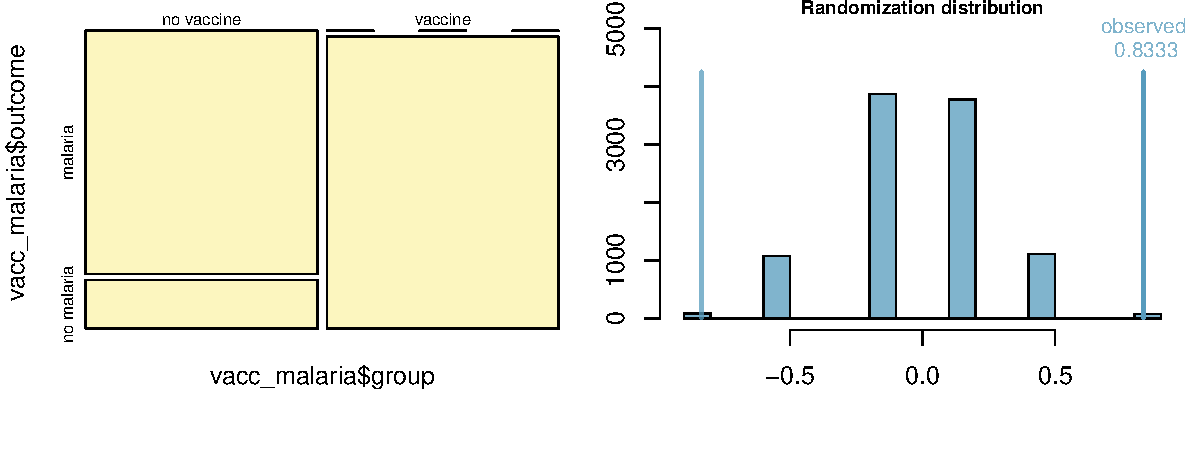
\includegraphics[width=0.75\textwidth]{figures/malaria/malaria}

\end{frame}

%%%%%%%%%%%%%%%%%%%%%%%%%%%%%%%%%%

\subsection{Comparing two proportions, large sample}

%%%%%%%%%%%%%%%%%%%%%%%%%%%%%%%%%%

\begin{frame}

\vfill

\app{App Ex 5.2}{See course website for details.}

\vfill

\end{frame}

%%%%%%%%%%%%%%%%%%%%%%%%%%%%%%%%%%%

\section{Summary}

%%%%%%%%%%%%%%%%%%%%%%%%%%%%%%%%%%%

\begin{frame}
\frametitle{Summary of main ideas}

\vfill

\begin{enumerate}

\item \nameref{mi1}

\item \nameref{mi2}

\item \nameref{mi3}

\end{enumerate}

\vfill

\end{frame}

%%%%%%%%%%%%%%%%%%%%%%%%%%%%%%%%%%%

\end{document}